\newcommand{\vect}[1]{#1} % no bold fonts
\newcommand{\dif}{\, d}
\newcommand{\disc}[1]{\left\llbracket {#1} \right\rrbracket}
\newcommand{\pd}{\partial}

\newcommand{\eps}{\epsilon}

\fenicschapter{Modeling evolving discontinuities}
              {Modeling evolving discontinuities}
              {Mehdi Nikbakht and Garth N. Wells}
              {nikbakht}

We present a framework for solving partial differential equations
with discontinuities in the solution across evolving surfaces. The
partition-of-unity/extended finite element approach is adopted, and
it is demonstrated that such methods can be used in combination with
a form compiler to generate equation-specific parts of a program. The
automated generation of code makes it straightforward to incorporate
discontinuities in formulations involving multiple fields, using both
Lagrange and non-Lagrange basis functions.  The approach is illustrated
through some salient code extracts.

\index{discontinuities}
%------------------------------------------------------------------------------
\section{Background}

The numerical solution of differential equations with discontinuities is
important in a range of fields. A notable example is the propagation of
cracks. Accounting for evolving discontinuities across \emph{a priori}
unknown surfaces in simulations using the finite element method poses
significant challenges.  Early attempts focused on mesh adaption to
construct meshes that conformed to the discontinuity surface.  More
recently, techniques have been developed that make it possible to include
discontinuous functions in a finite element basis, with the surface across
which the functions are discontinuous being independent of topology of
the underlying mesh. These techniques exploit the partition-of-unity
property of a standard finite element basis, and are known by a variety
of names, including the extended finite element method\index{extended
finite element method}, the partition of unity method\index{partition of
unity method} and the generalized finite element method\index{generalized
finite element method}.  Discontinuous solutions can evolve during the
solution of an equation, without the finite element mesh being adapted
to account for the discontinuity explicitly.

We present in this chapter an automated framework for modeling
evolving discontinuities which is based on the extended finite
element method. The extended finite element method is new
approach to model discontinuities independent of underlying mesh
\citep{BelytschkoBlack1999,MoesDolbowBelytschko1999,WellsSluys2001}.
An overview on the extended finite element method and similar methods
can be found in \citet{BabuskaBanerjeeOsborn2003}. The Unified Form
Language (\ufl) is used to express variational forms for problems with
discontinuous solutions, and extensions to the FEniCS Form Compiler
(\ffc) are developed for generating problem-dependent parts of the
computer code from \ufl{} input. To assemble and solve complete problems,
various tools are built upon the library \dolfin.  With the developed
framework, it is possible to use arbitrary combinations of different
finite element bases, and combinations of bases that may or may not
be discontinuous across a given surface. Our earlier effort in this
direction demonstrated the viability of the approach, but was limited in
scope \citep{NikbakhtWells2009}. Only continuous Lagrange basis function
functions were available, and only integration on cells was supported.
Moreover, the consistent abstractions and algorithms provided by {\ufl},
such as automatic differentiation, were not yet available. Less visible,
the entire library has been re-written to permit far greater flexibility.

In the remainder of this chapter, we review briefly the extended finite
element for modeling discontinuities and formulate it in such a way that
the computer input will resemble closely the mathematical description. The
software components used in the automated framework are then discussed,
as are aspects of the design, including interfaces. The approach is then
illustrated using code extracts for a range of examples.
The complete computer codes for partition of unity compiler and solver are available
at \url{https://launchpad.net/ffc-pum} and \url{https://launchpad.net/dolfin-pum}, respectively.
%------------------------------------------------------------------------------
\section{Partition-of-unity/extended finite element method}
%
Consider a domain $\Omega \subset \mathbb{R}^{d}$, where $1 \leqslant d \leqslant 3$,
that contains the surface~$\Gamma_{d}$ across which the function $u:
\Omega\backslash \Gamma_{d} \rightarrow \mathbb{R}$ is discontinuous
(see Figure~\ref{fig:nikbakht:domain}).
%
\begin{figure}
\begin{center}
  \def\svgwidth{8cm}
  \import{chapters/nikbakht/pdf/}{domain.pdf_tex}
\end{center}
\caption{Domain $\Omega$ intersected by a discontinuity
surface~$\Gamma_{d}$.}
\label{fig:nikbakht:domain}
\end{figure}
%
To denote functions that are evaluated at a surface, but by approaching
the surface from opposite sides of the surface, the subscripts `$+$' and
`$-$' will be used. The outward normal to $\pd \Omega$ and $\Gamma_{d}$
will be denoted by $\vect{n}$. The vector $\vect{n}$ is in the direction
of the `$+$' side. If we wish to find a function $u$ that
satisfies the Poisson equation:
%
\begin{align}
  - \Delta u &= f \quad {\rm in} \ \Omega \backslash \Gamma_{d}, \\
           u &= 0 \quad {\rm on} \ \pd \Omega, \\
  \nabla u_{+} \cdot \vect{n} &= q \quad {\rm on} \ \Gamma_{d},\\
  \disc{\nabla u} \cdot \vect{n} &= 0 \quad {\rm on} \ \Gamma_{d},
\end{align}
where $f: \Omega \rightarrow \mathbb{R}$ is a source term,
$q: \Gamma_d \rightarrow \mathbb{R}$ is the flux across discontinuity
surface~$\Gamma_d$ and $\disc{a} = a_{+} - a_{-}$.
Assuming that the flux on the discontinuity surface is given by $q =
q(\disc{u})$, the corresponding variational problem reads: find $u \in
H_{0}^{1}\brac{\Omega\backslash\Gamma_{d}}$ such that
%
\begin{equation}
  \int_{\Omega\backslash\Gamma_{d}}  \nabla u \cdot \nabla v \dif x
      + \int_{\Gamma_d} q(\disc{u})\disc{v} \dif s
      = \int_{\Omega} f v \dif x
\quad \foralls \ v \in H_{0}^{1}\brac{\Omega\backslash\Gamma_{d}}.
\label{eqn:nikbakht:poisson_discontinuous_variational}
\end{equation}
%
To compute approximate solutions to this problem, the task is to formulate
a suitable Galerkin finite element method that can accommodate the
discontinuous nature of the solution.

Consider a decomposition of the function $u$ according to
%
\begin{equation}
  u = \Bar{u} + \mathcal{H} \Hat{u},
\label{eqn:nikbakht:u_decomp}
\end{equation}
%
where $\Bar{u}: \Omega \rightarrow \mathbb{R}$ and $\Hat{u}: \Omega
\rightarrow \mathbb{R}$ are continuous functions, and $\mathcal{H}$ is
the Heaviside function centered at the surface across which $u$ exhibits
a jump.  We use the terminology `continuous' loosely for now, and for
simplicity we consider $\Hat{u}$ to be defined everywhere in~$\Omega$.
If $\mathcal{T}$ is a triangulation of the domain $\Omega$, consider
the finite element function spaces
%
\begin{align}
  \Bar{V}_{h} &= \bracc{\Bar{v}_{h} \in H^{1}_{0}(\Omega)
                    : \Bar{v}_{h} \in P_{k}(K) \ \foralls \ K \in \mathcal{T}},
\\
  \Hat{V}_{h} &= \bracc{\Hat{v}_{h} \in H^{1}_{0}(\Hat{\Omega})
                    : \Hat{v}_{h} \in P_{k}(K) \ \foralls \ K \in \Hat{\mathcal{T}}},
\end{align}
%
where $\Hat{\Omega}$ is the union of the supports of all finite element
functions whose support is intersected by the surface~$\Gamma_{d}$,
$\Hat{\mathcal{T}}$ in the restriction of $\mathcal{T}$ to $\Hat{\Omega}$
and $K$ is a finite element cell.  A finite dimensional analogue of the
decomposition in~\eqref{eqn:nikbakht:u_decomp} reads
%
\begin{equation}
  u_{h} = \Bar{u}_{h} + \mathcal{H} \Hat{u}_{h},
  \label{eqn:nikbakht:u_h_decomp}
\end{equation}
%
where $\Bar{u}_{h} \in \Bar{V}_{h}$ and $\Hat{u}_{h}
\in \Hat{V}_{h}$ ($\Hat{u}_{h} = 0$ for $\vect{x} \notin
\Hat{\Omega}$).  Decomposing a test function $v_{h}$ in the
same manner, a Galerkin version of the variational problem
in~\eqref{eqn:nikbakht:poisson_discontinuous_variational} reads: find
$(\Bar{u}_{h}, \Hat{u}_{h}) \in \Bar{V}_{h} \times \Hat{V}_{h}$ such that
%
\begin{multline}
     \int_{\Omega} \nabla \Bar{u}_{h} \cdot \nabla \Bar{v}_{h} \dif x
     + \int_{\Hat{\Omega}_{+}} \nabla \Hat{u}_{h} \cdot  \nabla \Bar{v}_{h} \dif x
     + \int_{\Hat{\Omega}_{+}}  \nabla \brac{\Bar{u}_{h} + \Hat{u}_{h}} \cdot \nabla \Hat{v}_{h} \dif x
     + \int_{\Gamma_d} q(\Hat{u}_h)\Hat{v}_h \dif s
\\
  =
   \int_{\Omega} f \Bar{v}_{h} \dif x
 + \int_{\Hat{\Omega}_{+}}  f \Hat{v}_{h} \dif x
      \quad \foralls \ (\Bar{v}_{h}, \Hat{v}_{h}) \in \Bar{V}_{h} \times \Hat{V}_{h},
\label{eqn:nikbakht:poisson_expanded_discontinuous_variational}
\end{multline}
%
where $\Hat{\Omega}_{+} \subset \Hat{\Omega}$ is the portion of
$\Hat{\Omega}$ on which $\mathcal{H} = 1$.
When presenting finite element function spaces
with discontinuities in Section~\ref{sec:nikbakht:examples}, the more compact
notation of the form
%
\begin{equation}
  V = \bracc{v_{h} \in H_{0}^{1}\brac{\Omega \backslash \Gamma_{d}}, \,
          v_{h}|_{K} \in P_{k}\brac{K \backslash \Gamma_{d}} \foralls K}
\end{equation}
%
will be used. The implementation of the discontinuous spaces expressed
using the above notation follows the approach described in this section.

In terms of finite element basis functions,
equation~\eqref{eqn:nikbakht:u_h_decomp} is expressed as follows:
%
\begin{equation}
  u_{h} = \sum_{i}^{n} \Bar{\phi}_{i} \Bar{u}_{i}
    + \sum_{j}^{m} \mathcal{H} \Hat{\phi}_{j} \Hat{u}_{j},
\label{eqn:nikbakht:basis_decomp}
\end{equation}
%
where $\Bar{\phi}_{i}$ and $\Hat{\phi}_{j}$ are the finite element basis
functions associated with $\Bar{V}_{h}$ and $\Hat{V}_{h}$, respectively,
and $\Bar{u}_{i}$ and $\Hat{u}_{j}$ are the regular and `enriched' degrees
of freedom, respectively. Note that the usual interpolation property
of finite element functions does not hold in the region of a discontinuity
surface. In practice $m \ll n$.

There are a number of issues that make the generation of computer
code for the extended finite element method more complex than for the
conventional finite element method.  A key point is that integration
schemes must be evaluated at runtime since it is necessary to perform
quadrature on both sides of discontinuity surface for intersected cells.
Moreover, for problems in which flux-like quantities are prescribed
on discontinuity surfaces, it is necessary to integrate terms on the
surface $\Gamma_{d}$.  Another issue is that the number of degrees of
freedom associated with each element is not constant and it depends on
the location of the discontinuity surface, and in the case of an evolving
discontinuity, this changes during a simulation.  The variable number
of cell degrees of freedom can make it difficult to generalize existing
finite element solvers to support partition-of-unity methods.

This section has demonstrated the use of a Heaviside enrichment via the
extended finite element method. It is possible to use other enrichment
functions in combination with the extended finite element method.
Commonly, functions that span the near-tip solution in linear elastic
fracture mechanics are used.  The scope of our work is limited to the
Heaviside function.
%------------------------------------------------------------------------------
\section{Software components}

In automating the generation of extended finite element models, we build
upon three key components from the \fenics{} project. Firstly, the Unified
Form Language (\ufl{}, Chapter~\ref{chap:alnes-1]}) is used to express variational
statements. Particular use is made of the concept of `enriched' spaces
and the \ufl{} concept of a `restriction'. The latter is the restriction
of functions to a particular entity sub-domain.  To generate code for a
finite element assembler (and additional helper functions), we develop
extensions of the \fenics{} Form Compiler (\ffc{}, Chapter~\ref{chap:logg-1})
for generating \ufc{}-compliant code. Finally, re-usable tools for the
implementation of extended finite element methods, including an interface
layer to transfer enriched degree of freedom data to the generated code,
function spaces and surface abstractions, are constructed upon \dolfin{}
(Chapter~\ref{chap:logg-2}).
%------------------------------------------------------------------------------
\subsection{Form language}

For the extended finite element method, it is necessary to define
function spaces that are restricted to subdomains, to define
functions which are restricted on discontinuity surfaces, and to define a
measure for surfaces to facilitate integration on surfaces.  \ufl{}
does not address these three issues explicitly, but it does provide the
necessary abstractions that can be used to communicate representations of
forms that involve discontinuous function spaces to a form compiler. We
use features of \ufl{}, but rely also on a form compiler to interpret
the \ufl{} representation appropriately.  The \ufl{} definition of a
problem is therefore an incomplete definition, with the form compiler
being relied upon to interpret various abstractions correctly. Therefore,
form compilers that support \ufl{} will not necessarily generate the
required code.

We define a discontinuous function space by restricting (informally)
a continuous function space by a measure~\emp{dc}. Motivated by
equation~\eqref{eqn:nikbakht:u_decomp}, we wish to locally enrich a
continuous function space with a space that contains a discontinuity. We
do this by adding continuous and discontinuous function spaces to create
an `enriched' space:
%
\begin{python}
Ec = FiniteElement("Lagrange", "tetrahedron", 2)
Ed = RestrictedElement(Ec, dc)
E  = Ec + Ed
\end{python}
%
In the above, \emp{Ec} is a regular scalar Lagrange finite element
on a tetrahedron of order two. \emp{Ed} is the restriction of the
space \emp{Ec} to the subdomain $\Hat{\Omega}$, and it will contain
a discontinuity. The geometry of the surface across which functions
are discontinuous will only be known at runtime, hence details of the
restriction can only be determined then. The expression \emp{E = Ec +
Ed} creates an enriched finite element. A more classical context in
which the enriched space concept in \ufl{} is used is for element-wise
bubble functions.  We note that construction of discontinuous UFL function
spaces in this manner is not unequivocal, but it is simple for the user.
The exact details of how the spaces are constructed does have a dependency
on the implementation. We feel that this is a limited price to pay in
return for ease of use.

Once an enriched finite element is defined, functions can be defined on
the enriched space. For example, enriched trial and test functions and
an enriched coefficient function are defined by:
%
\begin{python}
u = TrialFunction(E)
v = TestFunction(E)
f = Coefficient(E)
\end{python}
%
We can also restrict coefficients, test and trial functions
defined on discontinuous space to the positive or negative side of a
discontinuity. The \emp{jump} and \emp{average} of the function value
of $v$ across the surface is defined by:
%
\begin{python}
jump(v) = v('+') - v('-')
avg(v)  = [v('+') + v('-')]/2
\end{python}
%
respectively.

For the rest, variational forms can be expressed just as they are for
conventional problems using \ufl{}. In addition to the usual \ufl{}
syntax, \emp{dc} can be used to indicate integration of terms on a
discontinuity surface.  A number of complete examples of \ufl{} input
are presented in Section~\ref{sec:nikbakht:examples}.
%------------------------------------------------------------------------------
\subsection{FFC extensions}

To generate low-level code for an assembly library, extensions to \ffc{}
have been developed for performing tasks that are specific to the extended
finite element method.  Tasks that are specific to the extended finite
element method are:
%
\begin{itemize}
  \item Evaluation of element tensors for cells on which enriched
  functions are active;

  \item Evaluation of enriched finite element functions that do not
  satisfy the interpolation property; and

  \item Generation of \dolfin~ wrapper classes to aid in the
  initialization of enriched function spaces and data corresponding to
  the enriched degrees of freedom using discontinuity surfaces.
\end{itemize}
%------------------------------------------------------------------------------
\subsection{Assembler and solver}
%
The component for the assembly and solution of the finite element
equations is developed in C++ and builds on \dolfin{}. It is the most
complex of the necessary extensions. The main tasks of the solver are:
%
\begin{itemize}
  \item Management of data and tools related to the partition-of-unity
  method;

  \item Interaction with the code generated by the form compiler;

  \item Representation of surfaces;

  \item Extension of surfaces for evolving surface geometry; and

  \item Visualization of functions with discontinuities.
\end{itemize}
%
Some generic details of how these features are implemented are provided
in the next section.

%------------------------------------------------------------------------------
\section{Design and implementation}
%------------------------------------------------------------------------------
\subsection{Form compiler}

A small number of Python modules have been developed that extend FFC
for problems with discontinuities. Features that a specific to the
extensions are:
%
\begin{itemize}
  \item Generation of intermediate representations for forms with
  discontinuous function spaces;

  \item `Expansion transformer' to separate standard and enriched terms
  appearing in integrals if any coefficient defined on a discontinuous
  space exists; and

  \item Functions to to handle enriched entries in element tensors.
\end{itemize}
%
The extended form compiler simply imports \ffc{} modules for the
bulk of the functionality.
%------------------------------------------------------------------------------
\subsection{Interface between the generated code and the solver}

The code generated by the extended form compiler conforms to the
\ufc{} specification, hence an assembly function that supports \ufc{}
can be used without modification.  However, to evaluate various
objects, such as element tensors, the generated code must be aware
of the discontinuity surface. To support this within the framework
of a \ufc{}-compliant finite element assembler, the necessary \ufc{}
objects are constructed with a \emp{GenericPUM} object, and they store a
reference to this object.  \emp{GenericPUM} defines an abstract interface
through which the generated code can retrieve necessary data from the
solver library. \emp{GenericPUM}, together with the \ufc{} specification,
therefore define the interface for interactions between generated code
and the solver environment.

The member functions of \emp{GenericPUM} provide four basic types
of functionality. The first is degree of freedom manipulation, and
specifically management of the enriched degrees of freedom associated
with the partition-of-unity method.  This includes the tabulation of
enriched degrees of freedom and the local dimension of a cell tensor,
which can change during a simulation (such as as when a discontinuity
surface is extended). The second group includes member functions
of \emp{GenericPUM} interface that tabulate enrichment functions at
points (such as the Heaviside function for problems that involve a
discontinuity), which are needed when computing element tensors and
when interpolating functions at cell vertices. The \emp{GenericPUM}
interface also provides functions for modified quadrature rules. This
is essential when using non-polynomial enrichment functions, and in
particular discontinuous functions. For discontinuous functions, it is
important that a sufficient number of quadrature points are used on either
side of a discontinuity surface. \emp{GenericPUM} provides a function
that indicates when modified quadrature is required on a given cell or
facet, and it provides an interface for returning tailored quadrature
schemes. Finally, the \emp{GenericPUM} interface introduces some member
functions to update data related to the enriched degrees of freedom when
the discontinuity surfaces evolve.

The \emp{GenericPUM} interface is abstract, hence the generated code is
independent of various implementation details, such as the method by
which a discontinuity surface is represented and quadrature method on
intersected cells.

%------------------------------------------------------------------------------
\subsection{Assembler and solver}

The key classes that are developed upon \dolfin{} are a concrete
implementation of the \emp{GenericPUM} interface and the representation
of surfaces. To decouple the representation of surfaces from other
implementation details, an abstract base class \emp{GenericSurface} is
defined. The \emp{GenericSurface} interface provides various functions
for querying a surface object, such as whether a surface intersects
a cell.  It also provides an interface for returning quadrature
schemes on a surface, as this is intimately related to details of the
surface representation.  The use of the base class \emp{GenericSurface}
permits different surface representations to be used interchangeably
with the generated code. Surface representation is an active area
of research in the context of the extended finite element method (See
\citep{JagerSteinmannKuhl2008} for example), and the \emp{GenericSurface}
interface permits a high degree of flexibility in this respect.

In addition to concrete implementations of \emp{GenericPUM} and
\emp{GenericSurface}, a variety other low-level functionality is
implemented for performing various geometry operations, such as
sub-triangulation of finite element cells that are intersected by
a surface.

%------------------------------------------------------------------------------
\section{Examples}
\label{sec:nikbakht:examples}

Examples are presented in this section to demonstrate usage of
framework.  These examples aim to illustrate the generality in terms
modeling discontinuities in different equations using different basis
functions. Low-level code is generated from the compiler input by running
from the command-line:
%
\begin{bash}
ffcpum -l dolfin foo.ufl
\end{bash}

For each presented example the bilinear form $a$, the linear form $L$
and a function space $V$ are defined. The complete finite element problem
then involves: find $u_{h} \in V$ such that
%
\begin{equation}
  a(u_{h}, v_{h}) = L(v_{h}) \quad \foralls v_{h} \in V.
\end{equation}
%
For a nonlinear equation, the above is interpreted as the linearized
problem that is solved within a Newton iteration.

%------------------------------------------------------------------------------
\subsection{$H^{1}$-conforming primal approach to the Poisson equation}
%
As a canonical example, we present the Poisson equation in which the solution
$u$ is discontinuous across the surface $\Gamma_{d}$ and the flux across the
surface $ q = k\brac{u_{+} - u_{-}}$, where $k$ is a parameter.
For a conforming approach, the relevant function space is
%
\begin{equation}
  V = \bracc{v_{h} \in H_{0}^{1}\brac{\Omega \backslash \Gamma_{d}}, \,
          v_{h}|_{K} \in P_{k}\brac{K \backslash \Gamma_{d}} \foralls K}
\label{eqn:nikbakht:compact_discontinuous_space}
\end{equation}
%
and the bilinear and linear forms read
%
\begin{align}
  a\brac{u_{h}, v_{h}}
     &= \int_{\Omega \backslash  \Gamma_d} \nabla u_{h} \cdot \nabla v_{h} \dif x
       + \int_{\Gamma_{d}} k \disc{u_{h}} \disc{v_{h}}  \dif s,
\label{eqn:nikbakht:poisson_xfem_a}
\\
  L\brac{v_{h}} &= \int_{\Omega} f v_{h} \dif x,
\label{eqn:nikbakht:poisson_xfem_L}
\end{align}
%
where $f$ is a source term.

The form compiler input for this problem, in two dimensions, using linear
Lagrange elements is presented in Figure~\ref{code:nikbakht:Poisson}.
%
\begin{figure}
\begin{python}
# Define continuous and discontinuous spaces
elem_cont    = FiniteElement("CG", triangle, 1)
elem_discont = RestrictedElement(elem_cont, dc)

# Create enriched space
element = elem_cont + elem_discont

# Create test and trail functions
v, u = TestFunction(element), TrialFunction(element)

# Interface flux parameter and source term
k = Constant(triangle)
f = Coefficient(elem_cont)

# Create linear and bilinear forms
a = inner(grad(u), grad(v))*dx + k*jump(u)*jump(v)*dc
L = f*v*dx
\end{python}
\caption{{\ufl} input for the Poisson equation using a $H^{1}$-conforming
method with a discontinuous solution across a surface.}
\label{code:nikbakht:Poisson}
\end{figure}
%%
The code generated by the form compiler is used as input for a C++
solver. Discontinuity surfaces are defined in the solver environment.
An extract of the C++ solver is shown in
Figure~\ref{fig:nikbakht:poisson_c++}.  The C++ code is designed to
following the {\dolfin} style of mirroring mathematical abstractions
and keeping the code compact.  The code for the objects
\emp{Poisson::FunctionSpace}, \emp{Poisson::BilinearForm} and
\emp{Poisson::LinearForm} is problem specific and has been generated
by the form compiler, whereas the other elements appearing in
Figure~\ref{fig:nikbakht:poisson_c++} are standard {\dolfin} objects,
unless prefaced with the \emp{pum} namespace. Note that the function
space in the code extract is initialized with \emp{surfaces}, which is
a container of \emp{GenericSurface} objects. This is a convenience
wrapper for a \ufc{} function space, with \emp{GenericPUM} being
created internally from the surfaces, and then used to initialize the
\ufc{} objects.  Note also the use of \emp{pum::Function}, which is a
subclass of \emp{dolfin::Function} and implements primarily
restrictions of discontinuous coefficient functions for use in forms,
and interpolation of functions to cell vertices for use in
post-processing.
%
\begin{figure}
\begin{c++}
#include <dolfin.h>
#include <PartitionOfUnity.h>
#include "Poisson.h"

  . . .

int main()
{
  // Create mesh
  dolfin::UnitSquare mesh("mesh.xml.gz");
  . . .

  // Surface 0: A straight line (define by end points)
  std::pair<Point, Point> end_points0(p0_0, p0_1);
  pum::Surface d0(mesh, end_points0);

  // Surface 1: A curved line (define by end points and a level set function)
  std::pair<Point, Point> end_points1(p1_0, p1_1);
  const Shape1 shape1;
  pum::Surface d1(mesh, end_points1, shape1);

  // Add surfaces to an STL container
  std::vector<const pum::GenericSurface*>
       surfaces = boost::assign::list_of(d0)(d1);

  // Create function space with discontinuities across surfaces
  Poisson::FunctionSpace V(mesh, surfaces);

  // Create bilinear and linear Forms
  Poisson::BilinearForm a(V, V);
  a.k = k;
  Poisson::LinearForm L(V);
  L.f = f;

  // Create a linear variational problem and solve
  dolfin::VariationalProblem pde(a, L, bcs);
  pum::Function u(V);
  pde.solve(u);

  // Save solution to file for visualisation
  dolfin::File file("poisson.pvd");
  file  << u;

  // Save surfaces to file
  pum::VTKFile file_surface("surface.pvd");
  std::pair<std::vector<const GenericSurface*>,
            const dolfin::Mesh*> out_surfaces(surfaces, &mesh);
  file_surface << out_surfaces;
}
\end{c++}
\caption{C++ code extract for solver of the Poisson problem with
discontinuities in the solution. The notation resembles closely \dolfin{}
code for conventional problems.}
\label{fig:nikbakht:poisson_c++}
\end{figure}

A mesh with superimposed discontinuity surfaces and the computed
solution contours for this problem on a unit square domain
containing two disjoint discontinuity surfaces are shown in
Figure~\ref{fig:nikbakht:poisson_contours}.  For this case, $f = 1$
and $k = 1$.  Homogeneous Dirichlet boundary conditions are applied
along the bottom edge ($y = 0$). The remaining boundaries are flux-free.
The impact of the discontinuities on the computed solution contours can
be seen clearly in Figure~\ref{fig:nikbakht:poisson_contours}(b).
%
\begin{figure}
\begin{tabular}{cc}
  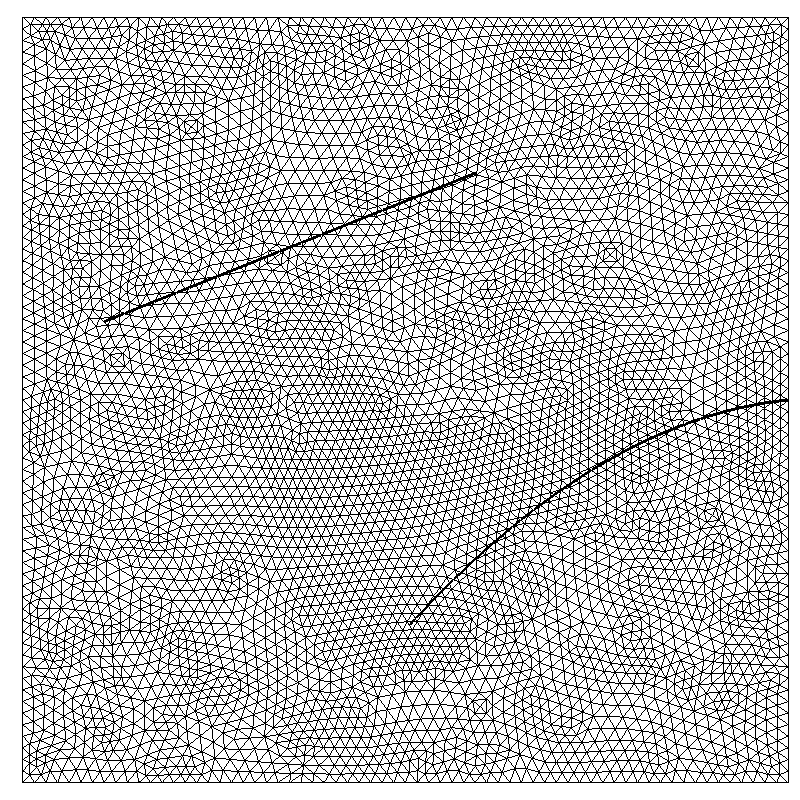
\includegraphics[height=0.45\textwidth]{chapters/nikbakht/png/mesh.png}
&
   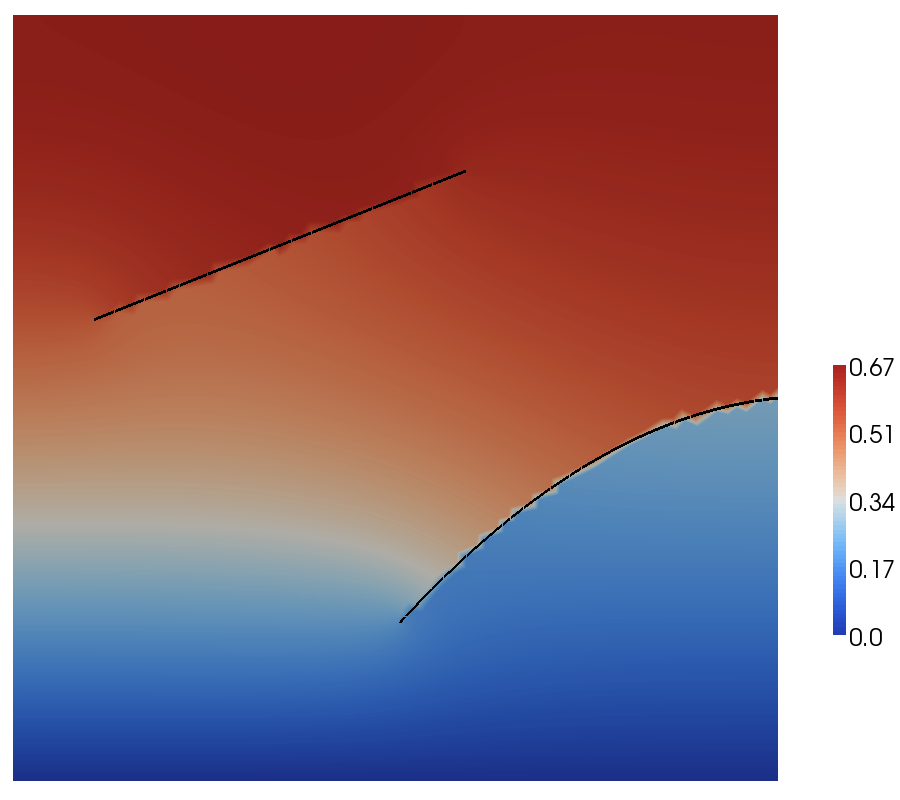
\includegraphics[height=0.45\textwidth]{chapters/nikbakht/png/result.png}
\\
(a) & (b)
\end{tabular}
\caption{Poisson problem in two dimensions: (a) mesh and discontinuity
surfaces and (b) solution contours.}
\label{fig:nikbakht:poisson_contours}
\end{figure}
%------------------------------------------------------------------------------
\subsection{$H(\rm div)$-conforming mixed approach to Poisson's equation}

\ffc{} supports a range of $H(\rm div)$ and $H(\rm curl)$ elements
that can be used in combination with other finite element types
\citep{RognesKirbyLogg2009}. These elements can also be used within the
context of the extended finite element method. To demonstrate this, \ufl{}
input for solving the Poisson equation with a discontinuity using the
$H(\rm div)$-conforming BDM element (see \citet{BrezziDouglasMarini1985}
and Chapter~\ref{chap:kirby-6}) for the flux and $L^{2}$-conforming Lagrange
functions for the scalar field is presented.  The relevant function
spaces for this problem read
%
\begin{align}
  V_{h} &= \bracc{\vect{\tau}_{h} \in H\brac{{\rm div}, \Omega\backslash\Gamma_{d}}, \,
         \vect{\tau}_{h}|_{K} \in \brac{P_{k}\brac{K \backslash \Gamma_{d}}}^{d} \foralls K},
\label{eqn:nikbakht:BDM_space}
\\
  W_{h} &= \bracc{\omega_{h} \in L^{2}\brac{\Omega}, \,
         \omega_{h}|_{K} \in P_{k-1}\brac{K \backslash \Gamma_{d}}\foralls K}.
\label{eqn:nikbakht:DG_space}
\end{align}
%
For homogeneous Dirichlet boundary conditions, the bilinear and linear
forms read:
%
\begin{align}
  a(\vect{\sigma}_{h}; u_{h}, \vect{\tau}_{h}; \omega_{h})
    &= \int_{\Omega\backslash\Gamma_{d}} \vect{\sigma}_{h} \cdot  \vect{\tau}_{h}
        - u_{h} (\nabla \cdot \vect{\tau}_{h}) + (\nabla \cdot \vect{\sigma}_{h}) \omega_{h} \dif x,
\\
  L(\vect{\tau}_{h}; \omega_{h}) &= \int_{\Omega} f \omega_{h}  \dif x.
\end{align}
%
Unlike the $H^{1}$-conforming Poisson example, this example implies that
$u_{h} = 0$ (weakly) on $\Gamma_{d}$ since the terms $\int_{\Gamma_{d}}
u_{h\pm} \vect{\tau}_{h\pm} \cdot \vect{n}_{\pm} \dif s$, which arise
from integration by parts, have been discarded.  This example therefore
demonstrates how the extended finite element method can be used to
apply Dirichlet-type conditions that do not conform to the mesh for
a mixed-method.

The form compiler input for this problem is presented in
Figure~\ref{code:nikbakht:mixed-Poisson}.  Note the distinction between
enriched and mixed elements.  The usual BDM and piecewise-constant
elements are `enriched' to incorporate a potential discontinuity (using
the summation sign), and the enriched spaces are then combined to create
a mixed finite element (using the multiplication sign).
%
\begin{figure}
\begin{python}
# Define continuous (cell-wise) spaces
BDM_c = FiniteElement("Brezzi-Douglas-Marini", "triangle", 1)
DG_c  = FiniteElement("Discontinuous Lagrange", "triangle", 0)

# Define discontinuous spaces
BDM_d, DG_d = RestrictedElement(BDM_c, dc), RestrictedElement(DG_c, dc)

# Create enriched spaces
BDM, DG = BDM_c + BDM_d, DG_c + DG_d

# Create mixed element
mixed_element = BDM * DG

# Trial and test functions
sigma, u = TrialFunctions(mixed_element)
tau, w   = TestFunctions(mixed_element)

# Source term
f = Coefficient(DG_c)

# Bilinear form and linear forms
a = dot(sigma, tau)*dx - u*div(tau)*dx + div(sigma)*w*dx
L = f*w*dx
\end{python}
\caption{Form compiler input for the mixed Poisson problem with
discontinuous~$u$ and~$\vect{\sigma}$.}
\label{code:nikbakht:mixed-Poisson}
\end{figure}

%------------------------------------------------------------------------------
\subsection{$L^{2}$-conforming discontinuous Galerkin approach to
linearized elasticity}

\ffc{} supports integration on interior facets, which makes
it possible to generate code for discontinuous Galerkin methods
\citep{OelgaardLoggWells2008}.  For a discontinuous Galerkin interior
penalty formulation of linearized elasticity with a discontinuity in
the solution across $\Gamma_{d}$, the relevant function space reads
%
\begin{equation}
 V = \bracc{\vect{v}_{h} \in \brac{L^{2}\brac{\Omega}}^{d}, \,
            \vect{v}_{h}|_K \in (P_{k}(K\backslash\Gamma_{d}))^{d} \ \foralls K}.
\end{equation}
%
For homogeneous Dirichlet boundary conditions and traction-free
discontinuity surfaces ($\vect{q} = \vect{0}$), the bilinear form reads:
%
\begin{multline}
 a(\vect{u}_{h}, \vect{v}_{h}) = \int_{\Omega \backslash \Gamma_{d}} \vect{\sigma}(\vect{u}_{h})
                                :  \nabla \vect{v}_{h} \dif x
 -  \int_{\Gamma_0} \disc{\vect{u}_{h}} \cdot \langle \vect{\sigma}(\vect{v}_{h}) \rangle \vect{n}_{+} \dif s
 - \int_{\Gamma_{0}} \langle \vect{\sigma}(\vect{u}_{h}) \rangle \vect{n}_{+} \cdot \disc{\vect{v}_{h}}  \dif s
\\
 + \int_{\Gamma_0} \frac{E \alpha}{h}  \disc{\vect{u}_{h}} \cdot \disc{\vect{v}_{h}} \dif s
 -  \int_{\pd \Omega} \vect{u}_{h} \cdot \vect{\sigma}(\vect{v}_{h})\vect{n} \dif s
\\
 - \int_{\pd \Omega} \langle \vect{\sigma}(\vect{u}_{h}) \rangle \vect{n} \cdot \vect{v}_{h}  \dif s
 + \int_{\pd \Omega} \frac{E \alpha}{h}  \vect{u}_{h} \cdot \vect{v}_{h} \dif s,
\end{multline}
%
and the linear form reads:
%
\begin{equation}
 L(\vect{v}_{h}) = \int_{\Omega} \vect{f} \cdot \vect{v}_{h} \dif x,
\end{equation}
%
where
$\vect{\sigma}(\vect{u})
= \mu(\nabla\vect{u} + (\nabla \vect{u})^{T} )
+ \lambda {\rm tr}(\nabla \vect{u}) \vect{I}$
is the stress tensor and $\mu$ and $\lambda$ are Lam\'e parameters,
$\vect{n}_{+}$ is the unit outward normal to a cell facet from the `$+$' side,
$\Gamma_0$ is the union of all interior cell facets,
$\langle a \rangle = (a_{+} + a_{-})/2$ is the  average operator on cell facets,
$\disc{\vect{b}} = \vect{b}_{+} - \vect{b}_{-}$ is the jump operator on cell facets,
$E$ is Young's modulus, $h$ is a measure of the cell size
and $\alpha > 0$ is a dimensionless penalty parameter that
is required for stability.
The form compiler input for this problem is presented in
Figure~\ref{code:nikbakht:dg-elasticity}. The necessary operators at cell facets
are implemented as part of \ufl{}. Integration over interior and exterior
facets is indicated by \emp{*dS} and \emp{*ds}, respectively.
%
\begin{figure}
\begin{python}
# Define continuous and discontinuous spaces
elem_cont    = VectorElement("DG", triangle, 2)
elem_discont = RestrictedElement(elem_cont, dc)
element      = elem_cont + elem_discont

# Create test and trial functions
v, u = TestFunction(element), TrialFunction(element)

# Compute material properties
E, nu     = 200000.0, 0.3
mu, lmbda = E / (2*(1 + nu)), E*nu / ((1 + nu) * (1 - 2*nu))

# Facet normal component, cell size and source term
n, h = element.cell().n, element.cell().circumradius
f = Coefficient(elem_cont)

# Penalty parameters
alpha = 4.0

# Stress
def sigma(v):
   return 2.0*mu*sym(grad(v)) \
  + lmbda*tr(sym(grad(v)))*Identity(v.cell().d)

# Bilinear form and linear forms
a = inner(sigma(u), grad(v))*dx \
  - inner(jump(u), avg(sigma(v))*n('+'))*dS \
  - inner(avg(sigma(u))*n('+'), jump(v))*dS \
  + (E*alpha/avg(h))*inner(jump(u), jump(v))*dS \
  - inner(u, sigma(v)*n)*ds \
  -inner(sigma(u)*n, v)*ds \
  + (E*alpha/h)*inner(u, v)*ds
L = inner(f, v)*dx
\end{python}
\caption{{\ufl} representation of the discontinuous Galerkin formulation of
linear elasticity equation with discontinuous $\vect{u}$ across~$\Gamma_{d}$.}
\label{code:nikbakht:dg-elasticity}
\end{figure}
%------------------------------------------------------------------------------
\subsection{Nonlinear Poisson-like equation}

We now consider a nonlinear problem that is solved using Newton's
method.  This example demonstrates the application of the automatic
differentiation feature of \ufl{} for a problem involving discontinuities.
The Poisson-like equation
%
\begin{equation}
  -\nabla \cdot \brac{1 + u^{2}} \nabla u = f
\end{equation}
%
on the domain $\Omega$, with $u = 0$ on $\partial \Omega$ and a flux-free
discontinuity surfaces ($q = \brac{1 + u^{2}} \nabla u \cdot \vect{n}
= 0$), can be phrased in a variational format as: find $u_{h} \in V$
such that
%
\begin{equation}
  F\brac{u_{h}; v_{h}}
    \equiv \int_{\Omega} \brac{1 + u_{h}^{2}} \nabla u_{h} \cdot \nabla v_{h}
      - f v_{h}  \dif x
    = 0 \quad \foralls \ v_{h} \in V,
\label{eqn:nikbakht:nonlinear_poisson}
\end{equation}
%
where $V$ is the space defined in
equation~\eqref{eqn:nikbakht:compact_discontinuous_space}.
The functional
$F$ is linear in $v_{h}$ but nonlinear in~$u_{h}$.  A nonlinear problem
posed in this format can be solved using Newton's method, in which $F$ is
driven to zero by solving a series of linear systems until a prescribed
tolerance is reached. The functional $F$, evaluated at the most recent
approximation of $u_{h}$, serves as the `linear form' (linear in $v_{h}$)
and the Jacobian of $F$, evaluated at the most recent approximation
of $u_{h}$, serves as the bilinear form (it is linear in $v_{h}$ and
$du_{h}$, where $du_{h}$ is the correction to the solution which is
computed by the Newton solver). Formally, the Jacobian is given by
%
\begin{equation}
  a\brac{u_{h}; du_{h}, v_{h}} = \left. \frac{dF\brac{u_{h}
      + \epsilon du_{h}; v_{h}}}{d \epsilon} \right|_{\epsilon=0}.
\label{eqn:nikbakht:nonlinear_poisson_J}
\end{equation}
%
Input to the form compiler will mirror this notation.

This example is relatively simple and the computation of the Jacobian
by hand is not onerous. However, for complicated nonlinear equations,
the derivation of an analytical expression for the Jacobian can be
lengthy and error prone (which is compounded by the extra complexity of
the extended finite element method).  For this task, exact automatic
differentiation is particularly attractive. Firstly, it eliminates a
source of errors.  Secondly, it means that if details of the equation of
interest are changed, then there is not need to re-evaluate the Jacobian
by hand. \ufl{} provides functionality for automatic differentiation,
and the directional derivative feature can be used to compute Jacobian
from a functional, with the Jacobian filling the role of the bilinear
form in the linearized system.

The \ufl{} input for the problem in
equation~\eqref{eqn:nikbakht:nonlinear_poisson} is shown in
Figure~\ref{fig:nikbakht:ufl_nonlinear_poisson}, where we have chosen
to use quadratic Lagrange functions.
%
\begin{figure}
\begin{python}
# Define continuous and discontinuous spaces
elem_cont    = FiniteElement("Lagrange", "triangle", 2)
elem_discont = RestrictedElement(elem_cont, dc)
element      = elem_cont + elem_discont

# Create test and trial functions
v, du = TestFunction(element), TrialFunction(element)

# Latest solution and source term
u, f = Coefficient(element), Coefficient(elem_cont)

# Bilinear form and Linear form
L = (1.0 + u**2)*inner(grad(u), grad(v))*dx - f*v*dx
a = derivative(L, u, du)
\end{python}
\caption{Form compiler input for the nonlinear Poisson-like equation. The bilinear
form (Jacobian) follows from differentiation of the linear form~\emp{L}.}
\label{fig:nikbakht:ufl_nonlinear_poisson}
\end{figure}

The trial function in this case is the iterative correction $du_{h}$,
and the most recent approximation of $u_{h}$ is provided as a coefficient
function to the forms.  Following from equation~\eqref{eqn:nikbakht:nonlinear_poisson_J},
the \ufl{} input the bilinear form (Jacobian) reads:
%
\begin{python}
a = derivative(L, u, du)
\end{python}
%
As with the other problems that we have presented, the generated code for
the linear and bilinear forms can be used in a \dolfin{}-based solver.
An extract of the DOLFIN/C++ code for solving this nonlinear problem is
presented in Figure~\ref{fig:nikbakht:c++_nonlinear_poisson}.
%
\begin{figure}
\begin{c++}
// Create function space
NonlinearPoisson::FunctionSpace V(mesh, surfaces);

// Solution function
pum::Function u(V);

// Create linear form
NonlinearPoisson::LinearForm F(V);
F.u = u; F.f = f;

// Create jacobian dF = F' (for use in nonlinear solver).
NonlinearPoisson::BilinearForm dF(V, V);
dF.u = u;

// Create and solve nonlinear variational problem
dolfin::VariationalProblem problem(F, dF, bc);
problem.solve(u);

// Save solution in VTK format
dolfin::File file("nonlinear_poisson.pvd");
file << u;
\end{c++}
\caption{C++ code extract for the nonlinear Poisson-like equation.}
\label{fig:nikbakht:c++_nonlinear_poisson}
\end{figure}
%------------------------------------------------------------------------------
\section{Summary}

It has been demonstrated that code for the extended finite element method
can be generated through a form compiler. \ufl{} provides the necessary
functionality to describe abstractly variational problems, and when paired
with a suitable form compiler computer code can be generated with the same
ease as for conventional finite element problems.  Automating aspects of
the extended finite element method poses a number of challenges that do
not feature in the conventional finite element method, such as adaptive
quadrature on cells intersected by a discontinuity surface and a variable
numbers of degrees of freedom at cells that are under the influence
of a discontinuity. By automating the generation of large parts of the
computer code, models that employ a variety of different finite element
basis functions, some with and others without discontinuous enrichment,
can be easily and rapidly developed.  Moreover, the generated code and
details of the adopted approach, such as the surface representation and
modified quadrature on intersected cells, can be decoupled via suitably
abstract class interfaces. This permits different implementation details
to be used without impacting on other aspects of the solver.
%------------------------------------------------------------------------------
